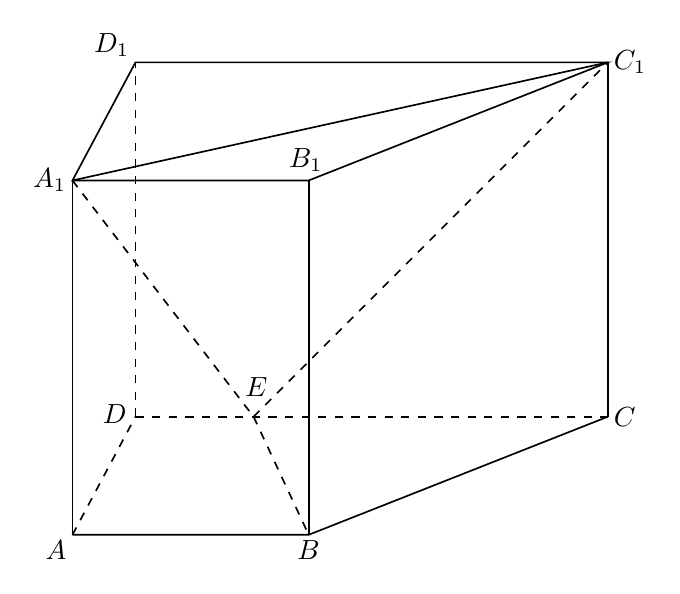
\begin{tikzpicture}[x=1cm,y=1cm,font=\normalsize,
  edge/.style={draw=black,solid,line width=.6pt},
  hide/.style={draw=black,dashed,line width=.6pt}]
% Right quadrangular prism ABCD-A1B1C1D1, E on CD
\coordinate (A) at (0.0,0.0);
\coordinate (B) at (3.0,0.0);
\coordinate (C) at (6.8000000000,1.5000000000);
\coordinate (D) at (0.8,1.5);
\coordinate (A1) at (0.0,4.5);
\coordinate (B1) at (3.0,4.5);
\coordinate (C1) at (6.8000000000,6.0000000000);
\coordinate (D1) at (0.8,6.0);
\coordinate (E) at (2.3000000000,1.5000000000);
% solid outline
\draw[edge] (A)--(B)--(C);
\draw[edge] (A)--(A1);
\draw[edge] (B)--(B1);
\draw[edge] (C)--(C1);
\draw[edge] (A1)--(B1)--(C1)--(D1)--cycle;
\draw[edge] (A1)--(C1);
% hidden base / vertical and auxiliary diagonals
\draw[hide] (A)--(D);
\draw[hide] (D)--(C);
\draw[hide] (D)--(D1);
\draw[hide] (A1)--(E);
\draw[hide] (E)--(C1);
\draw[hide] (E)--(B);
\node[below left,inner sep=2pt] at (A) {$A$};
\node[below,inner sep=2pt] at (B) {$B$};
\node[right,inner sep=2pt] at (C) {$C$};
\node[left,inner sep=2pt,xshift=-1pt,yshift=1pt] at (D) {$D$};
\node[left,inner sep=2pt] at (A1) {$A_{1}$};
\node[above,inner sep=2pt,xshift=-1pt,yshift=1pt] at (B1) {$B_{1}$};
\node[right,inner sep=2pt] at (C1) {$C_{1}$};
\node[above left,inner sep=2pt] at (D1) {$D_{1}$};
\node[above,inner sep=2pt,xshift=1pt,yshift=5pt] at (E) {$E$};
\end{tikzpicture}
